\section{Client Implementation}
\label{clientimpl}
Below we describe what the client side (Advert class) will look like.

\subsection{HTTP(S) Connections}
Since our client is implemented in pure Java, it is useful to make use of the
\texttt{java.net.URL} class, which allows us to make HTTP connections to the
App Engine. By creating an URL object like shown in Figure \ref{clientimpl-url}.

\begin{figure*}[ht] %[placement] where placement is h,t,b,p
\begin{center}
\begin{code}
URL url = new URL("http://ibis-advert.appspot.com/");
HttpURLConnection httpc = (HttpURLConnection) url.openConnection();
\end{code}
\caption{Opening an HTTP Connection.\label{clientimpl-url}}
\end{center}
\end{figure*}

Now it's possible with the use of the various functions in both classes to get
all information needed; like status-codes, HTTP Headers, and the message body.
This we will discuss below when we talk about the HTTP response.

In addition to HTTP connections, it is also possible in Java to make HTTPS
connections, however, this is not as straightforward as making HTTP connections.
To make an HTTPS connection we will need to import the
\texttt{java.security.Security} class (amongst others). In addition, if we look
at Figure \ref{clientimpl-https}, we see that the code adds us to the
\texttt{security.provider} list in \texttt{java.security}. After these lines of
code we will be able to make an HTTPS connection just like we did with making
HTTP connection above (i.e. \texttt{url.openConnection()}). All sample code is
fully operational at our branch in the JavaGAT SVN Repository .

\begin{figure*}[ht] %[placement] where placement is h,t,b,p
\begin{center}
\begin{code}
Security.addProvider(new com.sun.net.ssl.internal.ssl.Provider());

Properties properties = System.getProperties();

String handlers = System.getProperty("java.protocol.handler.pkgs");
if (handlers == null) { //nothing specified yet (expected case)
    properties.put("java.protocol.handler.pkgs",
        "com.sun.net.ssl.internal.www.protocol");
} 
else { //something already there, put ourselves out front
    properties.put("java.protocol.handler.pkgs",
        "com.sun.net.ssl.internal.www.protocol|".concat(handlers));
}
System.setProperties(properties);
\end{code}
\caption{Setting up an HTTPS Connection.\label{clientimpl-https}}
\end{center}
\end{figure*}

\subsection{HTTP POST method}
Secondly it is of great importance to create an HTTP POST request for both
authentication and sending data to the App Engine.

\subsubsection{Sending URL Encoded Strings}
The simplest option is to send a various number of URL encoded strings. An
example of making such an HTTP POST request can be seen in Figure
\ref{clientimpl-post}. We enable sending output to the connection just created,
calling \texttt{urlc.setDoOutput(true);}. After making this call we are able to
open an OutputStreamWriter to which we can write our POST data. Multiple fields are
separated by an ampersand, and variable names and values are separated by the
equal sign. In this example we write the author's name and content to an HTTP
POST request.

\begin{figure*}[ht] %[placement] where placement is h,t,b,p
\begin{center}
\begin{code}
/* Setting up POST environment. */
httpc.setRequestMethod("POST");
httpc.setDoOutput(true);
OutputStreamWriter out = new OutputStreamWriter(httpc.getOutputStream());

/* Writing POST data. */
out.write("author=bbn230&content=test");
out.close();
\end{code}
\caption{Making an HTTP POST request.\label{clientimpl-post}}
\end{center}
\end{figure*}

\subsubsection{Sending Binary Data}
In addition to just making HTTP post requests, it is also possible to send binary
data (commonly used for uploading files to web servers via HTTP). Again, this is
a step more difficult. We have to make sure the server expects a binary string of
data. This is shown in Figure \ref{clientimpl-binpost}. After the request has
been made, the content can be extracted from the message body by the server and
can be stored accordingly.

\begin{figure*}[ht] %[placement] where placement is h,t,b,p
\begin{center}
\begin{code}
/* Setting up POST environment. */
urlc.setDoOutput(true);
urlc.setRequestProperty("Content-Type", "application/octet-stream");
\end{code}
\caption{Making a binary HTTP POST request.\label{clientimpl-binpost}}
\end{center}
\end{figure*}

\subsubsection{Sending a Combination of Both}
\label{clientimpl-sending-both}

\paragraph{Multipart/Form-Data}
HTTP natively supports a standard for sending a combination of both URL encoded
Strings and binary data. This is specified in \emph{RFC1867} as
\emph{multipart/form-data}. Although this would seem perfect for our purposes, we
decided not to use this standard for sending a combination of URL encoded Strings
and binary data. RFC1867 specifies that every part of the message should be
seperated by a boundary, chosen by the client. The downside is that this boundary
cannot appear in the content of the payload. Since our payload can be virtually
anything, we decided to go a different direction, because otherwise we would have
to perform a linear search on all our data to see if a boundary token would
accidentally appear in our payload.

\paragraph{Custom Scheme}
Instead of using boundaries to define the start/end of our payload, we could make
use of special bytes which define the length of our payload. The layout of this
scheme is shown in Figure \ref{clientimpl-custom}. To begin with we start by
sending the length of the path, which is our first four bytes. Now the server
knows how many bytes the path will be (which is variable n), after which it knows
the meta data will follow. The meta data also starts with four bytes, indicating
the length (variable m). Finally, the object is sent, again, by sending the
object length as the first four bytes and the object (variable size p) right
after that.

\begin{figure*}[ht] %[placement] where placement is h,t,b,p
\begin{center}
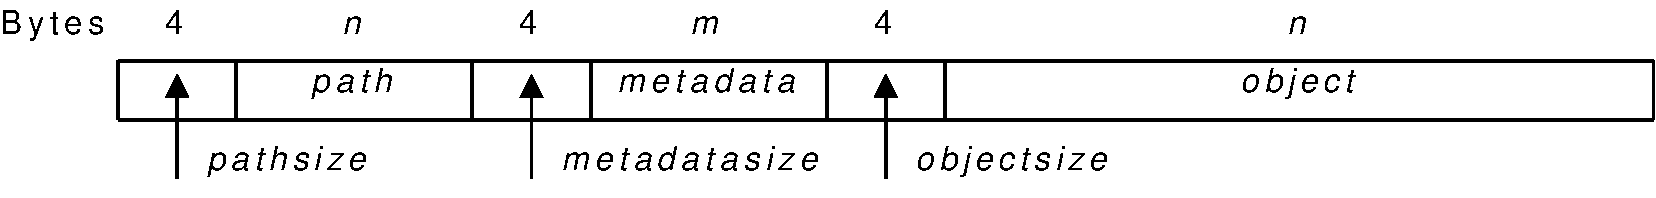
\includegraphics[width=12cm]{custom_payload.pdf} 
\caption{Custom Payload for Sending Binary Data.\label{clientimpl-custom}}
\end{center}
\end{figure*}

Our first attempt of sending the meta data was to structure it like this:
key1=value1: key2=value2: key3=value3: etc. At the client side, we would have to
escape actual content containing the equals sign or a colon, by placing a
backslash in front of them. We had to decode this again at the server side, to
make successful searches. Note that the earlier mentioned JSON is designed,
hence very effective, in sending such key-value pairs. If we take this even
further, JSON can do a lot more than just encoding key-value pairs.

\paragraph{JSON}
Besides serializing a MetaData object, JSON can actually serialize our whole
payload for us. This means that we don't have to work with neither boundaries,
as used in multipart/from-data, nor with payload sizes. Since both Java and
Python can use libraries which implements all JSON functionality, we won't
have to program a new mechanism of sending multiple Strings and binary data
in one request. 

To give the reader a small idea of how JSON works, we will try to encode te
payload above into a serial JSON String. The message consists out of three parts:
a path, meta data, and a binary object. So we will make a JSON array, with each
entry containing a part. The first part is just a String, which is a value for
the first entry. The second part is something more complicated, which we will
encode as a JSON obect, storing key-value pairs. The third entry again is a bit
more difficult, since we can only store Strings, numbers, booleans, and null.
That's why we formatted the binary object into a \emph{Base64} encoded
String\footnote{Base64 refers to a specific MIME content transfer encoding. It
encodes binary data by treating it numerically and translating it into a base 64
representation.}. The only downside is that Base64 encoding has a overhead of
about 1.35 of the original data length. For more information about the JSON
format, we refer to \cite{json-www}.

Once encoded, we can serialize the JSON array to a String (see Figure
\ref{clientimpl-json}), after which it will be sent to the server. We can decode
this String using simplejson at the server side, retrieving our JSON array back
(see Section \ref{serverimpl-simplejson}). 

\begin{figure*}[ht] %[placement] where placement is h,t,b,p
\begin{center}
\begin{code}
["/home/bboterm/app-engine/",{"key1":"value1","key2":"value2","key3":"value3"},
  "R0lGODlh(...)KSAAOw=="]
\end{code}
\caption{An example of a serial JSON array.\label{clientimpl-json}}
\end{center}
\end{figure*}

Note that all three parts need to be sent in one request, because suppose we send
all three parts in separate requests, requests could get lost, which would then
lead to inconsistencies.

\subsection{HTTP(S) Login}
Finally we want to `simulate' the login process through Google accounts. To
achieve this, we need the technique used above: making an HTTPS POST request.

\subsubsection{Google App Engine login page}
We have looked at the login page of a typical App Engine application, and we
have stripped the unnecessary HTML from the login form. As we can see from the
result shown in Figure \ref{clientimpl-loginform}, the login form is quite
comprehensive. The login form has a lot of extra (hidden and redundant) fields,
which we did not expect to find.

\begin{figure*}[ht] %[placement] where placement is h,t,b,p
\begin{center}
\begin{code}
<form id="gaia_loginform" 
action="https://www.google.com/accounts/ServiceLoginAuth?service=ah
    &amp;sig=d71ef8b8d6150b23958ad03b3bf546b7" 
  method="post"
  onsubmit="return(gaia_onLoginSubmit());">

<input type="hidden" name="ltmpl" value="gm">
<input type="hidden" name="continue" id="continue"
  value="http:// bbn230.appspot.com/_ah/login?
  continue=http://bbn230.appspot.com/" />
<input type="hidden" name="service" id="service" value="ah" />
<input type="hidden" name="ltmpl" id="ltmpl" value="gm" />
<input type="hidden" name="ltmpl" id="ltmpl" value="gm" />
<input type="hidden" name="ahname" id="ahname" value="Personal" />
<input type="text" name="Email"  id="Email" size="18" value="" />
<input type="password" name="Passwd" id="Passwd" size="18" />
<input type="checkbox" name="PersistentCookie" id="PersistentCookie" 
  value="yes" />
<input type="hidden" name='rmShown' value="1" />
<input type="submit" class="gaia le button" name="signIn" value="Sign in" />
<input type="hidden" name="asts" id="asts" value="">
</form>
\end{code}
\caption{Stripped down version of the App Engine
login page.\label{clientimpl-loginform}}
\end{center}
\end{figure*}

We are not sure what all hidden fields do, and if they are really necessary, but
simulating this login page by posting all this would make our HTTP POST request
quite large.

\subsubsection{Google Account Authentication API}
An alternative for simulating the login page is the \emph{Account
Authentication API} \cite{account-auth-api}. The Account Authentication API
comes in two forms. One form for installed \emph{Google Apps}
\cite{google-apps-www}, which is called \emph{ClientLogin}, the other is for Web
Apps, and is called \emph{OAuth} or \emph{AuthSub}.

\paragraph{ClientLogin}
Typically, ClientLogin is used for Installed applications that need to access
Google services protected by a user's Google or Google Apps. To make use of this
API, we will make a HTTP POST request to
\texttt{https://www.google.com/accounts/ClientLogin}, to which we send our
credentials as shown in Figure \ref{clientimpl-clientlogin}.

\begin{figure*}[ht] %[placement] where placement is h,t,b,p
\begin{center}
\begin{code}
StringBuilder content = new StringBuilder();
content.append("Email=").append(URLEncoder.encode("johndoe@gmail.com", 
  "UTF-8"));
content.append("&Passwd=").append(URLEncoder.encode("north23AZ", "UTF-8"));
content.append("&service=").append(URLEncoder.encode("ah", "UTF-8"));
content.append("&source=").append(URLEncoder.encode("Google App Engine", 
  "UTF-8"));
\end{code}
\caption{Preparing our ClientLogin credentials.\label{clientimpl-clientlogin}}
\end{center}
\end{figure*}

We created a Google Account for testing purposes and made a successful connection
using that account. The response of the ClientLogin is shown in Figure
\ref{clientimpl-clientlogin-response}.

\begin{figure*}[ht] %[placement] where placement is h,t,b,p
\begin{center}
\begin{code}
HTTP/1.1 200 OK
Content-Type: text/plain
Cache-control: no-cache, no-store
Pragma: no-cache
Expires: Mon, 01-Jan-1990 00:00:00 GMT
Date: Mon, 16 Mar 2009 14:07:25 GMT
X-Content-Type-Options: nosniff
Content-Length: 497
Server: GFE/1.3
----
SID=DQA(...)bjG
LSID=DQA(...)nSV
Auth=DQA(...)ub4
\end{code}
\caption{A response from ClientLogin.\label{clientimpl-clientlogin-response}}
\end{center}
\end{figure*}

Currently, `SID' and `LSID' are not used by the \emph{Google API}, so we just
need to extract the `Auth' value. Usually this value can be used directly on a
service its API (when providing a developer key), but unfortunately, the Google
App Engine is not listed in the Google data API library \cite{service-api}.
There is a workaround for still being able to connect to the App Engine, by
connecting to a App Engine's login page like Figure \ref{clientimpl-aelogin}.
In this example, \texttt{Auth} is a variable that contains the token acquired
by the example of Figure \ref{clientimpl-clientlogin-response}. 

\begin{figure*}[ht] %[placement] where placement is h,t,b,p
\begin{center}
\begin{code}
url = new URL("http://bbn230.appspot.com/_ah/login?auth="+ Auth);
\end{code}
\caption{Logging In for a Session Cookie.\label{clientimpl-aelogin}}
\end{center}
\end{figure*}

Connecting to this page will return a cookie with a session ID, just like the
one described in Section \ref{clientimpl-cookies}, only with a token called
`ACSID', with which we can identify ourselves to the App Engine for every
subsequent request.

\paragraph{AuthSub}
Web applications that need to access services protected by a user's Google or
Google Apps (hosted) account can do so using the Authentication Proxy service. To
maintain a high level of security, the proxy interface, called AuthSub, enables
the web application to get access without ever handling their users' account
login information. Before using, verify that the Google service to be accessed
supports the Authentication service. Some Google services may allow access only
to web applications that are registered and use secure tokens. We have not tried
AuthSub to authenticate ourselves at the App Engine. If the ClientLogin remains
to fail, we could consider AuthSub as our backup. We will not use it as our
primary authentication mechanism because if our users would want to install an
advert server, it would require extra effort, because they need to register
themselves first before this service can be used.

\subsubsection{Cookies}
Also, to maintain session with the server, we want to pass a session ID through
cookies. Also, this can be done through Java by setting the appropriate headers.
For example, if we want to send a cookie with the name ``SID'' and the content
``abcde'', we could code this in Java as shown in Figure
\ref{clientimpl-cookies-req}. This code will add the cookie to the HTTP request,
after which the response headers and body can be fetched.

\begin{figure*}[ht] %[placement] where placement is h,t,b,p
\begin{center}
\begin{code}
urlc.addRequestProperty("Cookie", "SID=abcde");
\end{code}
\caption{Sending cookies in Java.\label{clientimpl-cookies-req}}
\end{center}
\end{figure*}

\subsubsection{Persistent Authentication}
Because the authentication cookies, as provided by the Google App Engine,
generally expire after 24 hours. This means that, unless the user restarts the
Advert library, the user will receive an \emph{HTTP 403 Authentication} error,
once an Advert server runs over 24 hours consequently. 

To prevent the user from resetting the Advert server himself, we added a
\emph{Persistent Authentication} class. This class is actually a daemon thread,
which is created once the server has been authenticated. This server thread
parses the expiry date, which comes with the authentication cookie, and goes to
sleep 0.9 times the calculated expiry interval. As soon as the cookie is about
to expire, the daemon thread wakes up, and does a \texttt{NOOP} (NO OPeration)
call (i.e. a HTTP GET request of the main page), after which the App Engine
will automatically send a new authentication cookie and a new expiry date along
with it. Accordingly, we calculate the new expiry interval and go to sleep
again.

If the Advert service is used on a frequent basis, it could occur that by using
one of the Advert server's functions, a new (i.e. refreshed) cookie is sent
alongside the server response. If this is the case, the library will
automatically update the cookie present in the Persistent Authentication class,
so the daemon thread won't have to perform unnecessary \texttt{NOOP} calls.

The Persistent Authentication class is the only class where the authentication
cookie is stored. If a function wants to reference or update the authentication
cookie, \texttt{getCookie()} or \texttt{setCookie()} can be used respectively.

\subsection{HTTP Response}
After the HTTP request is sent, we are able to receive the HTTP response. To
begin with, we will download the response headers sent by the web server, after
which we can retrieve the body.

\subsubsection{Headers}
How to recieve the headers of an HTTP response is shown in Figure
\ref{clientimpl-headers}. Already, by receiving the response code, we can
distinguish errors from successful requests. Response codes starting with a 1 are
informational and those starting with a 2xx mean success. If the response code
is starting with a 3xx are used for redirection, and 4xx and 5xx are used for
errors (client and server respectively). For example: 200 stands for success, 403 for
authentication required, and 404 for not found.

\begin{figure*}[ht] %[placement] where placement is h,t,b,p
\begin{center}
\begin{code}
/* Retrieving headers. */
System.out.println(httpc.getResponseCode());
System.out.println(httpc.getRequestMethod());
for (int i = 0; httpc.getHeaderField(i) != null; i++) {
    System.out.println(httpc.getHeaderField(i));
}
\end{code}
\caption{Retrieving HTTP response headers.\label{clientimpl-headers}}
\end{center}
\end{figure*}

After checking the response code, we can retrieve additional headers. In our case
(using the App Engine as our web server), we have listed an example of receiving
a succesful response (Figure \ref{clientimpl-200}). Again, a status header is
sent, followed by the server type, the date, and some other info. Note that
``Content-Length'' can be really useful to determine our buffer size in the next
step.

\begin{figure*}[ht] %[placement] where placement is h,t,b,p
\begin{center}
\begin{code}
HTTP/1.0 200 OK
Server: Development/1.0
Date: Wed, 11 Mar 2009 11:25:05 GMT
Cache-Control: no-cache
Content-Type: image/gif
Content-Length: 18006
\end{code}
\caption{Example of HTTP response headers.\label{clientimpl-200}}
\end{center}
\end{figure*}

\subsubsection{Cookies}
\label{clientimpl-cookies}
A `special' type of HTTP header that can be retrieved from sending an HTTP
request are cookies. Just like all the other headers, it is retrieved with the
code stated above. When printed to screen, it will look similar to the request
shown in Figure \ref{clientimpl-cookies-resp}. This code above is taken from
retrieving the URL \texttt{http://www.google.nl/}. As you can see, this cookie
consists out of multiple parts, but would normally be stored as one cookie in your
browser. In this case, the cookies name is ``PREF'', and its content is
``ID=8f3c26(\ldots)zrigB6''. Finally it comes with an expiration time and date,
a path, and a domain. This information will be needed when we want to authenticate
ourselves to the App Engine.

\begin{figure*}[ht] %[placement] where placement is h,t,b,p
\begin{center}
\begin{code}
HTTP/1.1 200 OK
Cache-Control: private, max-age=0
Date: Wed, 11 Mar 2009 11:57:38 GMT
Expires: -1
Content-Type: text/html; charset=ISO-8859-1
Set-Cookie: 
  PREF=ID=8f3c262a9b38330e:TM=1236772658:LM=1236772658:S=L2ORt13rUlzrigB6; 
  expires=Fri, 11-Mar-2011 11:57:38 GMT; path=/; domain=.google.nl
Server: gws
\end{code}
\caption{An HTTP response including cookies.\label{clientimpl-cookies-resp}}
\end{center}
\end{figure*}

\subsubsection{Message Body}
Once we've received all headers and parsed them accordingly, we are able to get
the actual body. As we can see from Figure \ref{clientimpl-body}, the most
important thing is getting the stream, provided by the \texttt{getInputStream()}
function. After we have done this, we can basically do anything with our
InputStream. In this case we print it to the console, but we could also save it
in a buffer and manipulate it, or write it do disk, etc. After we are done
receiving the InputStream, we close the InputStream, effectively closing the
connection.

\begin{figure*}[ht] %[placement] where placement is h,t,b,p
\begin{center}
\begin{code}
BufferedReader in = 
  new BufferedReader(new InputStreamReader(httpc.getInputStream()));
String inputLine;

while ((inputLine = in.readLine()) != null) {
    System.out.println(inputLine);
}
in.close();
\end{code}
\caption{Retrieving the HTTP response's body.\label{clientimpl-body}}
\end{center}
\end{figure*}

